\chapter{\IfLanguageName{dutch}{Stand van zaken}{State of the art}}
\label{ch:stand-van-zaken}

% Tip: Begin elk hoofdstuk met een paragraaf inleiding die beschrijft hoe
% dit hoofdstuk past binnen het geheel van de bachelorproef. Geef in het
% bijzonder aan wat de link is met het vorige en volgende hoofdstuk.

% Pas na deze inleidende paragraaf komt de eerste sectiehoofding.

De literatuurstudie geeft een beeld van welke programma’s in dit onderzoek worden opgenomen. Voordat deze IDEs worden besproken, wordt er eerst een definitie opgesteld van de IDE en de source code editor, om het verschil duidelijk te maken. Daarna volgt er een geschiedenis van het opkomen van de IDE alsook de nood van de moderne IDE in de ontwikkelingsomgeving. Als laatste worden de aanbevolen systeemvereisten aangehaald zodat er al een beeld gevormd kan worden van hoe de verschillende IDEs zullen presteren.

\section{\IfLanguageName{dutch}{IDE en Source Code Editor}{IDE and Source Code Editor}}
\label{sec:IDE-codeEditor}

De termen IDE en source code editor, meestal verkort tot code editor, worden vaak door elkaar gebruikt. Er is daarentegen een functioneel verschil tussen deze twee termen. Het verschil wordt verduidelijkt met de volgende definitie:

“An integrated development environment (IDE) is software for building applications that combines common developer tools into a single graphical user interface (GUI). An IDE typically consists of a Source code editor,  Local build automation, Debugger.” \autocite{RedHat2018}

De code editor maakt dus integraal deel uit van de IDE. Deze laatste bevat daarnaast namelijk andere tools zoals een geïntegreerde compiler/interpreter, build-automatisatie, een debugger, versiecontrole, een test framework en soms nog andere tools. Voorbeelden van IDEs in dit onderzoek zijn Visual Studio, Eclipse en IntelliJ.

Onder code editor wordt verstaan dat dit een grafische tekst editor is met extra features zoals syntax markering, indentatie, auto-voltooiing en bracket matching. Hieruit kan ook afgeleid worden dat code editors lagere hardware vereisten hebben doordat deze minder features hebben. Moderne code editors maken vaak gebruik van plug-ins of extensions om meer functionaliteiten van de IDE aan te bieden. Maar in het algemeen bieden ze dit niet standaard aan en moet de gebruiker dit zelf configureren.

\begin{figure}[h!]
    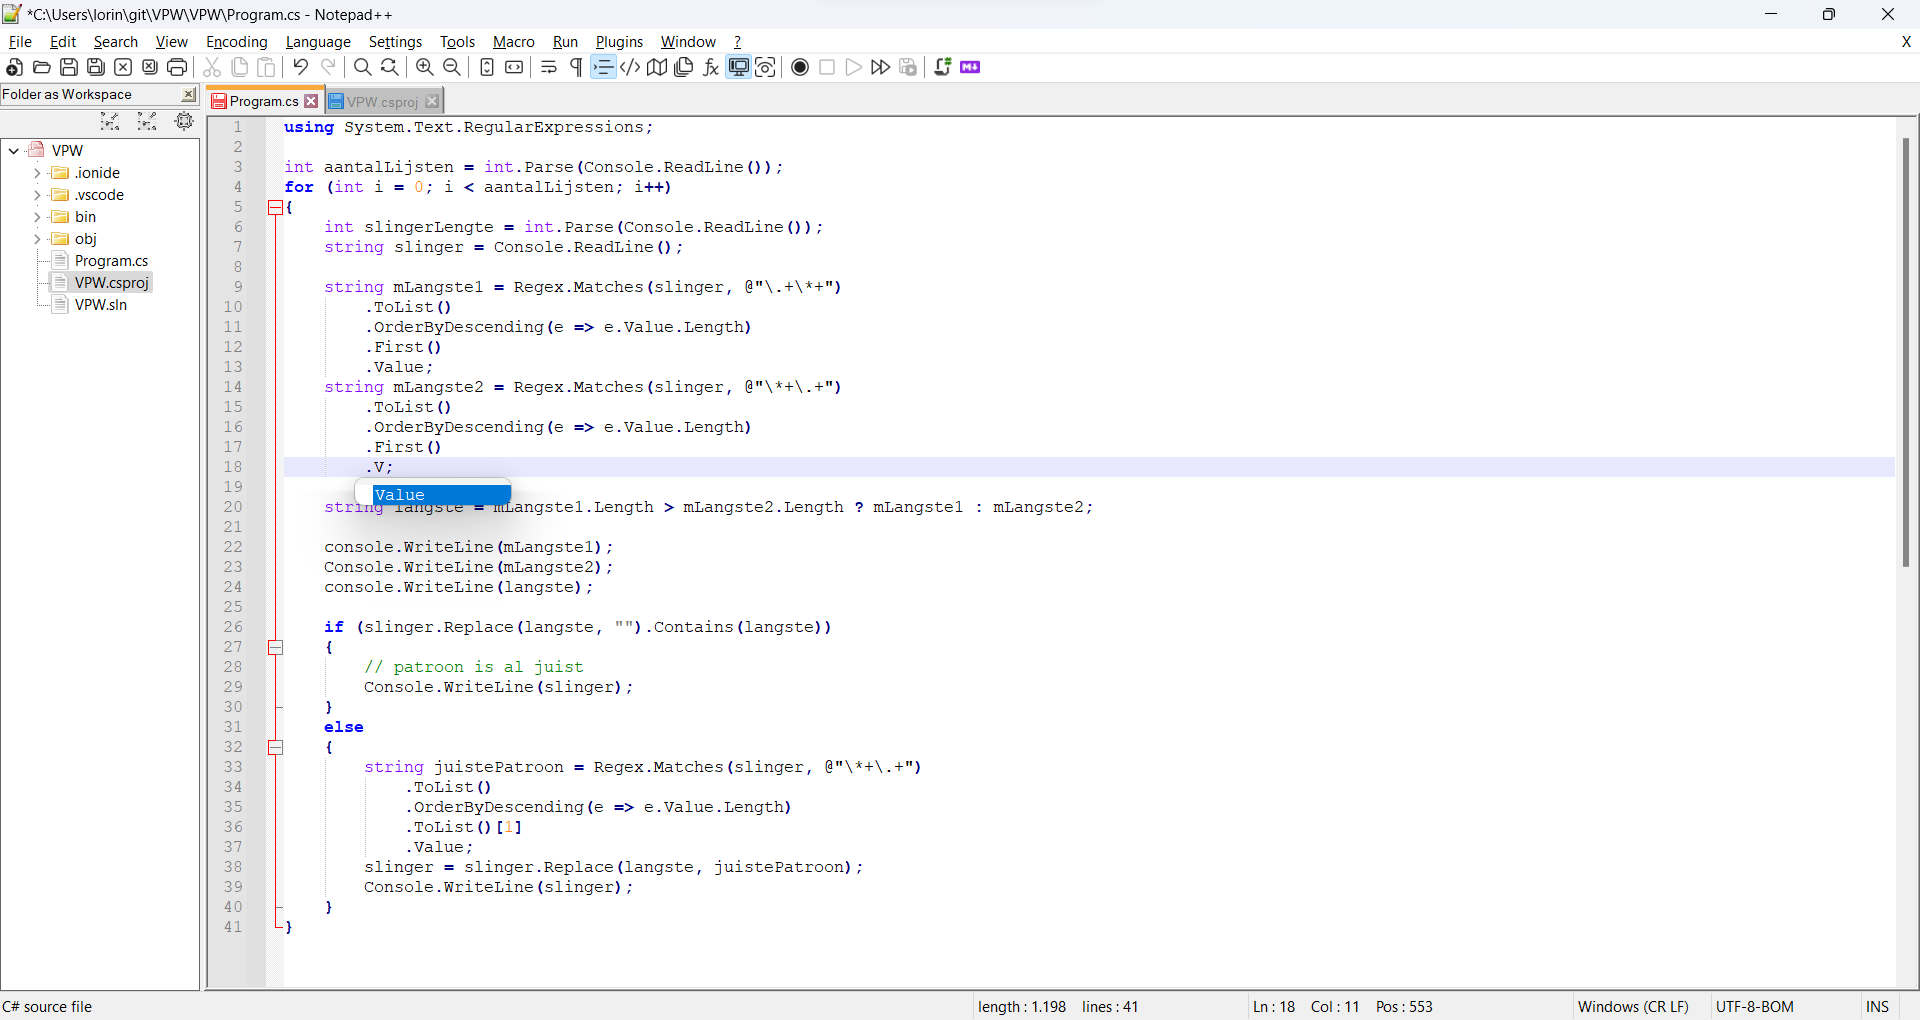
\includegraphics[width=\linewidth]{CodeEditor.png}
    \caption{De Notepad++ code editor}
    \label{fig:codeEditor}
\end{figure}

\begin{figure}[h!]
    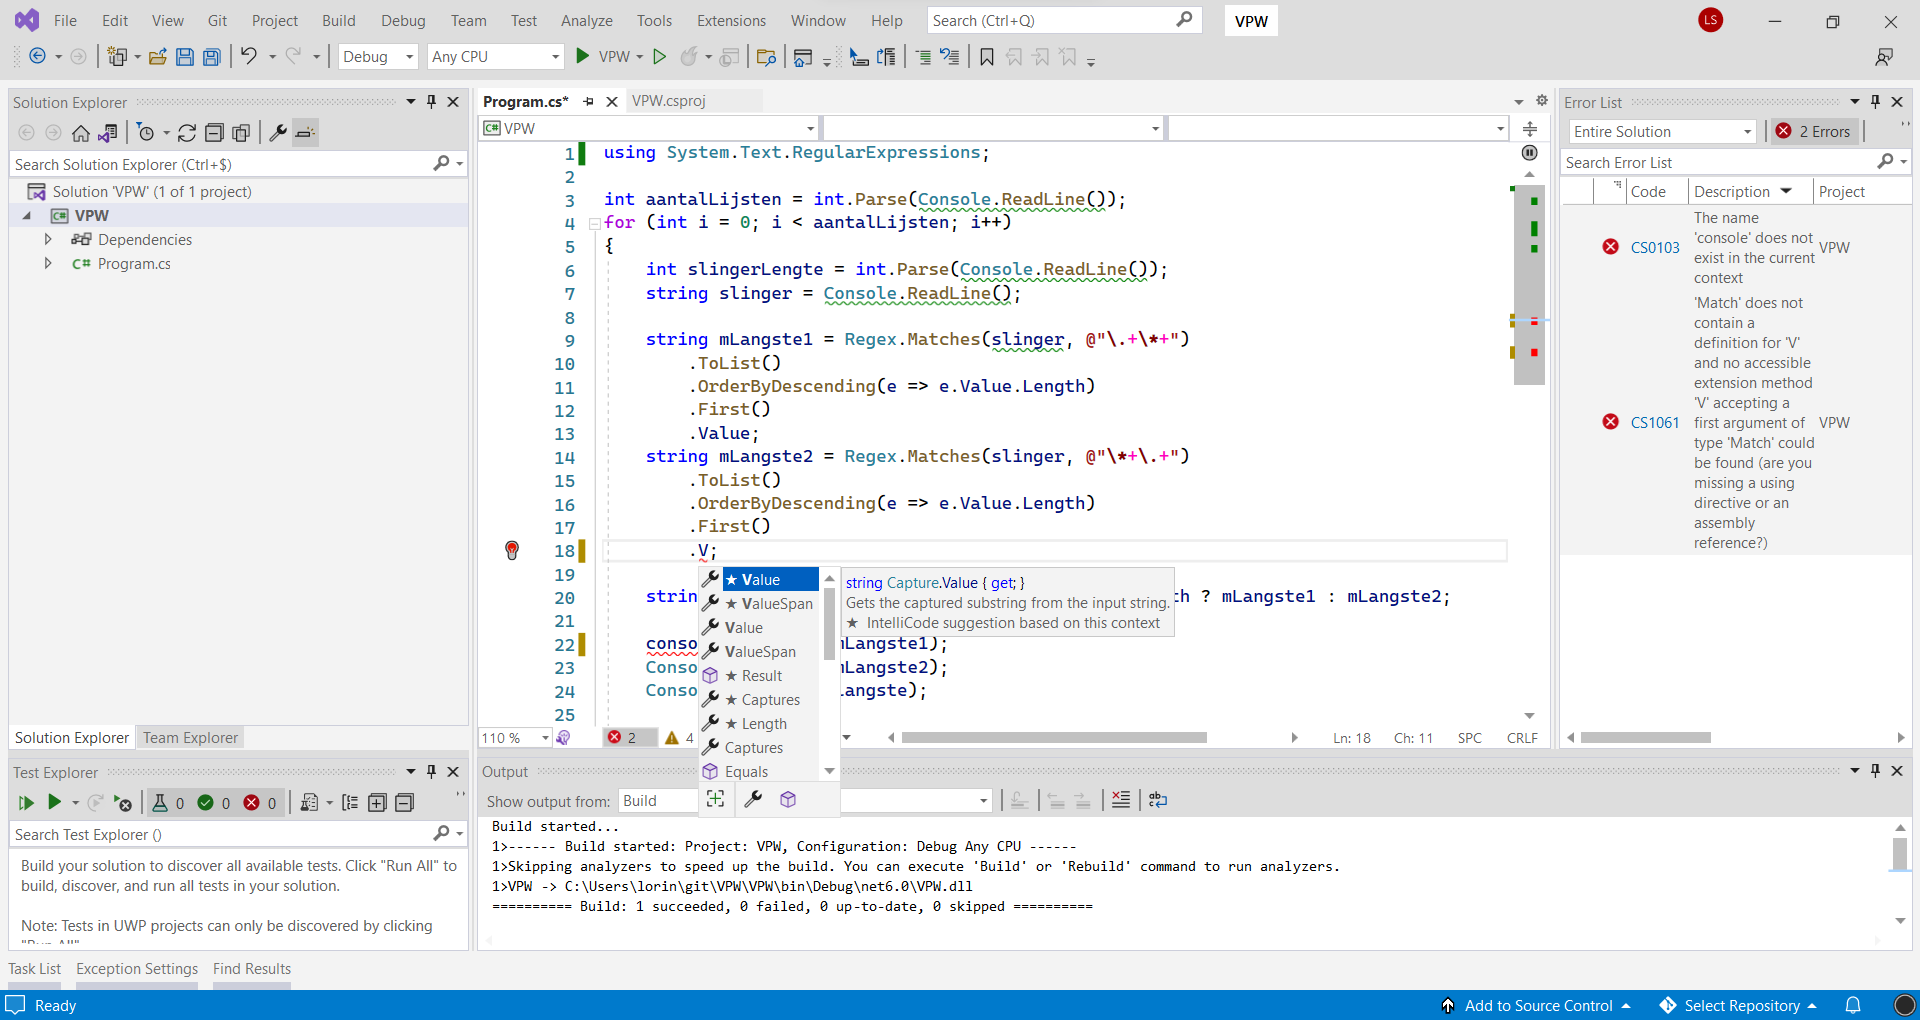
\includegraphics[width=\linewidth]{IDE.png}
    \caption{De Visual Studio IDE}
    \label{fig:IDE}
\end{figure}

Als illustratie zijn 2 afbeeldingen van hetzelfde project gegeven om het verschil in functionaliteit tussen de code editor en de IDE te verduidelijken. Op het eerste gezicht zijn deze vrij gelijkend, een tekst editor die centraal staat met daarrond wat vensters en knoppen. Maar bij nader inzicht is het duidelijk dat de IDE meer aanbiedt, zoals sterkere syntax markering(meer sleutelwoorden worden gekleurd), context bewuste aanvulling (het menu onderaan de V), error controle(lijst van errors en rood onderlijnde code), build en run uitvoer, testen, debugging via breakpoints…

\section{\IfLanguageName{dutch}{Ontstaan van de IDE}{Origin of the IDE}}
\label{sec:IDE-ontstaan}

De eerste IDE is ontwikkeld in 1980, nadat programmeertalen overschakelden naar ontwikkeling via de console. Dit was hiervoor niet mogelijk omdat de eerste software geprogrammeerd werd met ponskaarten. De eerste computertaal die bewerkt kon worden met een IDE was Dartmout basic. Deze IDE was gelimiteerd in functionaliteit en werd niet bestuurd met een GUI, maar met console commando’s. Het doel van deze eerste IDE, net zoals nu, was om de productiviteit van de programmeur te verhogen. \autocite{JAXenter2018}

Dit gebeurde door de verschillende tools die een programmeur nodig had om software te maken, te combineren. Dit zorgde voor een reductie in ontwikkelingstijd omdat in de oude workflow veel manuele taken zaten. Eerst werd het programma opgesteld in een standaard tekst editor. Daarna werd het bestand met de geschreven code door de compiler vertaald en werden de errors die deze teruggaf manueel op papier overgezet. Daarna werd de cyclus voltooid door terug naar de tekst editor te gaan om deze errors op te lossen. Dit was natuurlijk een zeer inefficiënte workflow. 

De eerste IDEs hadden wel problemen, ze waren bijvoorbeeld moeilijk in gebruik en hadden een grote leercurve, soms was zelfs professionele training nodig. Dit zorgde ervoor dat ze niet tot hun volledige potentieel gebruikt werden, of zelfs helemaal niet. Uit onderzoek van \textcite{Kline2005} werd er opgemerkt dat 70\% van CASE tools(computer-assisted software engineering tools, waaronder IDEs vallen) een jaar na aankoop niet meer gebruikt werden. Hier kwam dan ook bij dat de aanschaffingskosten heel hoog waren, deze konden oplopen tot \$20,000 per ontwikkelaar.

Samen met de steeds groeiende hardware mogelijkheden en de verspreiding van Windows kwamen de GUI gebaseerde IDE’s op. Deze werd gepionierd door Visual Basic, de eerste in de markt met drag en drop functionaliteit. De volgende IDE die de markt voortstuwde was Visual Studio met zijn eerste uitgave in 1997. Dit was een van de eerste IDEs die niet enkel bedoeld was om voor 1 specifieke computertaal te werken maar voor verschillende tegelijk. 

\section{\IfLanguageName{dutch}{Nood van IDEs in de moderne ontwikkelingsomgeving}{Need of IDEs in the modern developement environement}}
\label{sec:IDE-nood}

Nu na jarenlange ontwikkeling is de IDE een belangrijke tool in het arsenaal van programmeurs, en zijn er vele verschillende opties voor elke taal en framework. Als er naar volgend onderzoek van \textcite{Tidelift2019} gekeken wordt, kan er opgemerkt worden dat het merendeel van de ontwikelaars tijd in de IDE wordt doorgebracht. Hierbij zijn de bevindingen dat er 32\% effectief besteed wordt aan het schrijven van nieuwe code, wat in de IDE uitgevoerd wordt. Daarnaast wordt er 19\% van de tijd aan code management en 12\% aan testen besteed, wat mogelijk is gemaakt door de geïntegreerde refactoring en test tools van IDEs. Samen betekende dit dat 63\% van de ontwikelaars tijd in de IDE wordt doorgebracht, hieruit volgt dus de nood voor performante IDEs.

\section{\IfLanguageName{dutch}{Prominente IDEs}{Prominent IDEs}}
\label{sec:IDE-prominent}

Er zijn momenteel een groot aanbond van IDE’s verkrijgbaar, sommige betalend en sommige gratis. De meeste IDEs focussen zich op lichtelijk andere doeleinden, sommigen leggen zicht toe op 1 specifieke programmeertaal en bieden hier dan diepgaande integraties voor, waar andere minder specifiek gaan en de gebruiker zelf de verschillende talen moet configureren. De verschillende IDEs hebben ook verschillende groottes van gebruikersgroepen, de ene is al populairder als de andere. Deze studie zal zich bezighouden met de 4 meest populaire en hun gratis/betalende tegenhangers genomen zoals onderzocht in de \textcite{StackOverflow2021} devolpper survey. 

\subsection{Visual Studio Code}
Visual Studio Code\footnote{https://code.visualstudio.com/}, afgekort tot VS Code, is een open source code editor ontwikkeld door Microsoft. Deze editor is volledig gratis en heeft geen betalende opties. VS Code is een van de jongere editors, met zijn originele uitgave in 2015. VS Code is een voorbeeld van dog fooding\footnote{https://twitter.com/code/status/907328551157768192} waar Microsoft hun eigen software gebruikt voor hun ontwikkeling. 

VS Code is een lightweight editor wat inhoudt dat de standaard configuratie een kleine installatiegrootte heeft en snel in opstart is. Dit gaat natuurlijk wel gepaard dat standaard aangeboden functionaliteiten van deze editor beperkt is. Dit kan wel verholpen worden met het grote aanbod van plug-ins. Op de Visual Studio Marketplace zijn er momenteel 30.000 plug-ins\footnote{https://marketplace.visualstudio.com/search?target=VSCode} beschikbaar. Deze extensions voegen functionaliteit doe die gaan van thema’s en customisatie, tot programeer taal ondersteuning, refactorings, en extra features. De additie van deze extensions betekend wel dat de editor geleidelijk aan trager wordt als er meer bijkomen, dit is dan vooral merkbaar in de start tijd performantie. 

\subsection{Visual Studio }
Visual Studio\footnote{https://visualstudio.microsoft.com/vs/}, meestal met een jaar als versie postfix bv Visual Studio 2022, is een mature IDE met verschillende versies en jarenlange updates. Deze IDE is ontwikkeld door Microsoft en heeft zijn originele uitgave in 1997 met versie 97, momenteel is de nieuwste versie 2022. Visual Studio heeft een gratis Community versie beschikbaar voor studenten, academici, open source developers en kleine bedrijven. Deze versie bevat de meeste features, met een klein gebrek aan testing, profilering tools en minder integratie met Azure services. Voor grote bedrijven(jaarlijkse omzet groter dan \$1 miljoen) en bedrijven die nood hebben aan deze features bestaan dan de Professional en Enterprise versies die respectievelijk maandelijks \$45 en \$250 kosten\footnote{https://visualstudio.microsoft.com/vs/compare/} .

Visual Studio is een echte IDE, niet een code editor, dit betekend dat er diepgaande integratie is met het ontwikkelingsproces van de ondersteunde talen, van ontwerp, programmeren, testen tot productie en publicatie. Hiervoor bestaan er verscheidene tools voor die standaard toegankelijk zijn. Dit komt wel met extra gewicht en de bestandsgrote, processorkracht, ram vereisten zijn groter. Ook het achtergrond verbruik en de opstarttijd zijn hoger dan die van een code editor. 

Visual Studio heeft ook extensies voor extra functionaliteiten en customisatie. Sommige van de extensies worden aangeboden door Microsoft zelf, maar het merendeel wordt gemaakt door open-source developers. Het aanbod van plug-ins is kleiner als dat van VS Code, 1286\footnote{https://marketplace.visualstudio.com/search?target=VS\&vsVersion=vs2022} voor de nieuwste versie 2022. De meeste extensies zijn gratis maar er bestaan ook betalende. Een voorbeeld hiervan is ReSharper, deze extensie voegt nog diepgaandere code analyse en refactorings tools toe aan Visual Studio.

\subsection{Eclipse}
Eclipse\footnote{https://www.eclipse.org/eclipseide/2022} is een open source IDE ontwikkeld door eerst IBM en daarna de Eclipse foundation. Het doel van het project was een performante IDE bouwen die Visual Studio zou eclipsen. Eclipse heeft een rijke geschiedenis van verschillende versie met de initiële uitgave in 2001. Eclipse heeft net zoals VS Code een plug-in gebaseerde architectuur. Dit is wel minder merkbaar aangezien dat de standaard aangeboden functionaliteiten meer compleet zijn als in VS Code. Het aantal plug-ins momenteel beschikbaar op de marketplace telt 1496\footnote{https://marketplace.eclipse.org/}. Eclipse is volledig gratis, afgezien van bepaalde betalende extensies, en is mogelijk gemaakt door donaties vanuit de ontwikkelaars gemeenschap.

Eclipse is vooral gefocust op ontwikkeling met Java en is een van de populairste IDEs voor deze taal. Het was ook de officiële ontwikkelomgeving voor Android, voor deze veranderde naar Android Studio. Naast Java is er ook ondersteuning beschikbaar voor andere talen met zoals PHP C, C++, C\# Rust en vele anderen. Deze ondersteuning wordt aangeboden als individuele extensions.

\newpage

\subsection{IntelliJ IDEA}
IntelliJ IDEA\footnote{https://www.jetbrains.com/idea/} is een IDE in uit wijde aanbod van Jetbrains. Deze editor bestaat al lang met de eerste uitgave in 2001. Het was de eerste IDE die bij Jetbrains ontwikkeld werd,  waarna ze zouden verdergaan door meerder IDES te ontwikkelen voor verschillende programmeertalen. IntelliJ is gefocust op programmeertalen draaiend op de Java virtual machine(JVM) met ondersteuning voor Java, Scala, Groovy, Android en Kotlin

De community versie van IntelliJ is gratis en open source en bevat de belangrijkste features. De betalende Ultimate versie bevat extra ondersteunde programmeertalen en frameworks\footnote{https://www.jetbrains.com/products/compare/}. De prijs van de Ultimate versie is jaarlijks €500.

\subsection{Notepad++}
Notepad++\footnote{https://notepad-plus-plus.org/} is een code editor die in ontwikkeling is sinds 2003. Het project was gestart door Don Ho die ontevreden was met de performantie van andere editors. Het heeft de mogelijkheden om code te bewerken, heeft syntax markering en heeft gelimiteerde auto aanvulling, maar heeft geen geïntegreerde run en debug mogelijkheden. Deze kleine functieset kan juist een voordeel zijn, omdat er soms de nood is voor een simpele, makkelijk te leren editor die snel in gebruik is en weinig plaats vereist. 

Notepad++ biedt heeft net zoals de meeste editors plug-in ondersteuning. Momenteel zijn er 163 plug-ins\footnote{https://github.com/notepad-plus-plus/nppPluginList/blob/master/doc/plugin\_list\_x86.md} beschikbar op de nppPluginList. Notepad is volledige gratis en word financieel ondersteund door donaties. 

\newpage

\section{\IfLanguageName{dutch}{Opgegeven hardware vereisten}{Required hardware}}
\label{sec:IDE-prominent}

\begin{table}[h!]
    \begin{tabular}{lllll}
        & CPU         & Ram     & Opslag  & OS                       \\
        Notepad++     & 1.3 GHz & 0.5 GB   & 100 MB   & Win           \\
        VS Code       & 1.6 GHz & 1 GB     & 500 MB   & Win, Lin, Mac \\
        Eclipse       & 1.5 GHz & 1 GB     & 1 GB     & Win, Lin, Mac \\
        IntelliJ      & Modern  & 2–8 GB   & 3.5–5 GB & Win, Lin, Mac \\
        Visual Studio & 1.8 GHz & 4–16 GB  & 20-50 GB & Win          
    \end{tabular}
    \caption{Opgegeven hardware vereisten}
    \label{fig:requirementsTable}
\end{table}

Zoals te zien in bovenstaande tabel\footnote{https://www.getpcapps.com/software/development/notepad-plus-plus-code-editor-installer-setup-windows.html}\footnote{https://code.visualstudio.com/docs/supporting/requirements}\footnote{https://www.tabnine.com/blog/intellij-idea-vs-eclipse/}\footnote{https://www.jetbrains.com/help/idea/installation-guide.html}\footnote{https://docs.microsoft.com/en-us/visualstudio/releases/2022/system-requirements} zijn de opgegeven vereisten zeer uiteenlopend. De code editors(Notepad++ en VS Code) hebben vrij lichte vereisten en de IDEs (Eclipse, IntelliJ, Visual Studio) vereisen meer van het systeem. Dit zou kunnen betekenen dat de IDEs trager zijn op hardware met mindere specificaties en dat de code editors hier sneller zijn. Op krachtigere systemen is het afhankelijk van de IDE hoe goed die omgaan met de hardware middelen en hoe performant die uiteindelijk zal zijn. Dit is wat dit onderzoek tracht te onderzoeken.
